\documentclass{beamer}

\mode<presentation> {


%\usetheme{default}
%\usetheme{AnnArbor}
%\usetheme{Antibes} 
%\usetheme{Bergen}
%\usetheme{Berkeley}
%\usetheme{Berlin}
%\usetheme{Boadilla}
%\usetheme{CambridgeUS}
%\usetheme{Copenhagen}
%\usetheme{Darmstadt}
%\usetheme{Dresden}
%\usetheme{Frankfurt}
%\usetheme{Goettingen}
%\usetheme{Hannover}
%\usetheme{Ilmenau}
%\usetheme{JuanLesPins}
%\usetheme{Luebeck}
\usetheme{Madrid}
%\usetheme{Malmoe}
%\usetheme{Marburg}
%\usetheme{Montpellier}
%\usetheme{PaloAlto}
%\usetheme{Pittsburgh}
%\usetheme{Rochester}
%\usetheme{Singapore}
%\usetheme{Szeged}
%\usetheme{Warsaw}
%\usecolortheme{albatross}
%\usecolortheme{beaver}
%\usecolortheme{beetle}
%\usecolortheme{crane}
%\usecolortheme{dolphin}
%\usecolortheme{dove}
%\usecolortheme{fly}
%\usecolortheme{lily}
%\usecolortheme{orchid}
%\usecolortheme{rose}
%\usecolortheme{seagull}
%\usecolortheme{seahorse}
%\usecolortheme{whale}
%\usecolortheme{wolverine}

%\setbeamertemplate{footline} % To remove the footer line in all slides uncomment this line
%\setbeamertemplate{footline}[page number] % To replace the footer line in all slides with a simple slide count uncomment this line

%\setbeamertemplate{navigation symbols}{} % To remove the navigation symbols from the bottom of all slides uncomment this line
}

\usepackage{graphicx} % Allows including images
\usepackage{booktabs} % Allows the use of \toprule, \midrule and \bottomrule in tables
\usepackage{amsmath}
\usepackage{amssymb}
\usepackage{mathrsfs}
\usepackage{caption}
\usepackage{subcaption}
\usepackage{bbm} 
\usepackage{xcolor}
% \usepackage{natbib}
\usepackage[backend=biber, citestyle=apa, bibstyle=authoryear]{biblatex}
\addbibresource{NL_PF_QR.bib}
%----------------------------------------------------------------------------------------
%	TITLE PAGE
%----------------------------------------------------------------------------------------

\title[Quantile Production Functions]{Proxy Variable and Dynamic Nonlinear Estimation of Production Function Updates}

\author{Justin Doty} % 
\institute[] % Your institution as it will appear on the bottom of every slide, may be shorthand to save space
{
\\  
\medskip % Your email address
}
\date{\today} % Date, can be changed to a custom date

\begin{document}

\begin{frame}
\titlepage % Print the title page as the first slide
\end{frame}

%----------------------------------------------------------------------------------------
%	PRESENTATION SLIDES
%----------------------------------------------------------------------------------------

%------------------------------------------------
\section{First Section} % Sections can be created in order to organize your presentation into discrete blocks, all sections and subsections are automatically printed in the table of contents as an overview of the talk
%------------------------------------------------

\subsection{Subsection Example} % A subsection can be created just before a set of slides with a common theme to further break down your presentation into chunks

\begin{frame}
\frametitle{Introduction: Random Coefficient Model}
\begin{itemize}
\item Consider the random coefficient gross output production function (in logs)
\begin{equation} \label{pfrc}
    y_{it}=\beta_{0}(\eta_{it})+\beta_{k}(\eta_{it})k_{it}+\beta_{l}(\eta_{it})l_{it}+\beta_{m}(\eta_{it})m_{it}+\omega_{it}
\end{equation}
where $y_{it}$ denotes output, $l_{it}$ denotes labor input for firm $i$ at time $t$, $k_{it}$ denotes capital input, $m_{it}$ denotes material input, $\omega_{it}$ is unobserved productivity and $\eta_{it}$ denotes an iid shock to production.
\item If the production function is strictly increasing in $\eta_{it}$ then the conditional quantile of \eqref{pfrc} are
\begin{equation}
Q_{\tau}(y_{it}|\mathcal{I}_{it})=\beta_{0}(\tau)+\beta_{k}(\tau)k_{it}+\beta_{l}(\tau)l_{it}+\beta_{m}(\tau)m_{it}+\omega_{it}
\end{equation}
where $\mathcal{I}_{it}$ is the firm's information set at time $t$ which is independent of $\eta_{it}$.
\item In this specification, $\omega_{it}$ is a location-shifter of the conditional output distribution
\end{itemize}
\end{frame}

%------------------------------------------------------------------------------------

\begin{frame}
\frametitle{Random Coefficient Model}
\begin{itemize}
\item Doty and Song (2020) show how to identify and estimate this simple linear random coefficient model by extending the control variable approach of \cite{Levinsohn2003} of a value-added production function
\item I will briefly review our approach here. They assume the following
\textbf{Assumption 1}
\begin{enumerate}
	\item The production function $y_{it}=f_{t}(k_{it}, l_{it}, \omega_{it}, \eta_{it})$ is strictly increasing in $\eta_{it}$
	\item The firm's information set at time $t$ includes current and past productivity shocks $\{\omega_{it}\}_{t=0}^{t}$, but does not include past productivity shocks $\{\omega_{it}\}_{t=t+1}^{\infty}$. $\eta_{it}$ is independent of $\mathcal{I}_{it}$
	\item Firm's productivity shocks evolve according to a first-order Markov process
	\begin{equation}
	\omega_{it}=\rho\omega_{it-1}+\xi_{it}
	\end{equation}
	where the iid productivity innovations $\xi_{it}$ are independent of $\mathcal{I}_{it-1}$.\\
	We require that $P[\xi_{it}\leq F_{\xi}^{-1}(\tau)|\mathcal{I}_{it-1}]=P[\xi_{it}\leq F_{\xi}^{-1}(\tau)]=\tau$
\end{enumerate}
\end{itemize}
\end{frame}

%------------------------------------------------------------------------------------

\begin{frame}
\frametitle{Random Coefficient Model}
\textbf{Assumption 1 continued}
\begin{enumerate}
	\item Firms accumulate capital according to
	\begin{equation}
	    K_{it}=\kappa_{t}(I_{it-1}, K_{it-1}).
	\end{equation}
	where $K_{it-1}$ and $I_{it-1}$ denote previous period capital and investment
	\item Firm's intermediate input demand function is given by $m_{it}=m_{t}(k_{it}, \omega_{it})$
	\item The intermediate input demand function $m_{t}(k_{it}, \omega_{it})$ is strictly increasing in $\omega_{it}$
\end{enumerate}
\begin{itemize}
	\item We invert intermediate input demand $\omega_{it}=m^{-1}(k_{it}, m_{it})$ and substitute into the production function. We treat $m_{t}^{-1}$ as a nonparametric function $(k_{it}, m_{it})$. We then have:
	\begin{equation} \label{qpf1st}
		y_{it}=\beta_{k}(\eta_{it})k_{it}+\beta_{l}(\eta_{it})l_{it}+m_{t}^{-1}(k_{it}, m_{it})=\beta_{l}(\eta_{it})l_{it}+\Phi(k_{it}, m_{it}, \eta_{it})
	\end{equation}
\end{itemize}
\end{frame}

%------------------------------------------------------------------------------------

\begin{frame}
\frametitle{Random Coefficient Model}
\begin{itemize}
	\item Using Assumption 1 we have the following identification condition for the first stage:
		\begin{equation}
			P\big(y_{it}\leq \beta_{l}(\tau)l_{it}+\Phi(k_{it}, m_{it}; \tau)\big|\mathcal{I}_{it})=\tau
		\end{equation}
	\item We use a linear approximation $\Phi(k_{it}, m_{it}, \eta_{it})=\beta_{k}(\eta_{it})k_{it}+\beta_{m}(\eta_{it})m_{it}$ so we can estimate $\beta_{l}(\tau)$ and $\Phi(k_{it}, m_{it}, \tau)$ using linear quantile regression.
	\item We write a second stage identification condition in only the $\xi_{it}$ component, similar to \cite{Ackerberg2015} by concentrating out the constant $\beta_{0}(\tau)$ and $\rho$. For a hypothetical guess of $\beta_{k}(\tau)$ we can write
	\begin{equation}
		\tilde{\omega}_{it}=\beta_{0}(\tau)+\omega_{it}=y_{it}-\hat{\beta}_{l}(\tau)l_{it}-\beta_{k}(\tau)k_{it}=\hat{\Phi}(k_{it}, m_{it}; \tau)-\beta_{k}(\tau)k_{it}
\end{equation}
\end{itemize}
\end{frame}

%------------------------------------------------------------------------------------

\begin{frame}
\frametitle{Random Coefficient Model}
\begin{itemize}
	\item We estimate the AR(1) model with a constant so that
	\begin{equation}
	Q_{\tau}(\tilde{\omega}_{it}|\mathcal{I}_{it-1})=\alpha+\rho(\hat{\Phi}(k_{it-1}, m_{it-1}; \tau)-\beta_{k}(\tau)k_{it-1})+F_{\xi}^{-1}(\tau)
	\end{equation}
	\item We estimate $(\alpha+F_{\xi}^{-1}(\tau), \rho)$ using the procedure of \cite{He1997} called Restricted Regression Quantiles (RQQ)
		\begin{enumerate}
			\item First, a median regression of $\hat{\Phi}(k_{it}, m_{it}; \tau)-\beta_{k}(\tau)k_{it}$ on $\hat{\Phi}(k_{it-1}, m_{it-1}; \tau)-\beta_{k}(\tau)k_{it-1}$ to obtain estimates of $\rho$ so that it does not vary over $\tau$
			\item Second, let $\hat{\xi}_{it}=\hat{\Phi}(k_{it}, m_{it}; \tau)-\beta_{k}(\tau)k_{it}-\hat{\rho}(\hat{\Phi}(k_{it-1}, m_{it-1}; \tau)-\beta_{k}(\tau)k_{it-1})$. Then take the $\tau$th quantile of $\hat{\xi}_{it}$ as an estimate for $\hat{\alpha}+\hat{F}_{\xi}^{-1}(\tau)$
		\end{enumerate}
		\item The idea is to eliminate the Quantile Crossing problem by estimating $\rho$ separately 
		\item Since they do not vary over $\tau$, slope estimates are often poor if using quantile regression, especially at the tails
\end{itemize}
\end{frame}

%------------------------------------------------------------------------------------

\begin{frame}
\frametitle{Quantile Crossing Solution}
\begin{itemize}
	\item Other than to avoid the problem of the writing a moment condition that corresponds to the joint distribution of $\eta_{it}$ and $\xi_{it}$ I have no theoretical justification for using the RQQ for concentrating out moment conditions in $\xi_{it}$
	\item Generally, quantile crossing is a finite sample problem that goes away in the limit.
	\item Typically this problem makes charts hard to interpret as crossing can occur in certain areas of the sample space
	\item For example a predicted 95th percentile of the response could be smaller than the 90th percentile which is impossible
	\item The RQQ method enforces monotonicity, but is also inefficient compared to estimating quantiles simultaneously
	\item This method also looked good for Monte Carlo simulations (next slide) in this paper. However, applying this methodology to the data has been a pain
\end{itemize}
\end{frame}

%------------------------------------------------------------------------------------
\begin{frame}
\frametitle{Proxy Variable Monte Carlo Results}
\begin{figure}[ht]
\centering
\includegraphics[width=7cm, height=7cm]{/Users/justindoty/Documents/Research/Dissertation/Production_QR_Proxy/Code/Monte_Carlo/LP_Coefficient_Plot.png}
\end{figure}
\end{frame}

%----------------------------------------------------------------------------

\begin{frame}
\frametitle{Random Coefficient Model}
\begin{itemize}
	\item Therefore, we have the following identification condition
		\begin{equation}
		P[\hat{\xi}_{it}(\beta_{k}(\tau))\leq \hat{F}_{\xi}^{-1}(\tau)|\mathcal{I}_{it-1}]=P[\hat{\xi}_{it}(\beta_{k}(\tau))\leq \hat{F}_{\xi}^{-1}(\tau)]=\tau
		\end{equation}
		where $\mathcal{I}_{t-1}$ should include a constant and other instruments such as inputs determined in the prior period
	\item This can be represented by conditional moment restrictions
		\begin{equation} \label{conditional}
			\mathbb{E}[\mathbbm{1}\{\hat{\xi}_{it}(\beta_{k}(\tau))- \hat{F}_{\xi}^{-1}(\tau)\leq 0\}-\tau|\mathcal{I}_{it-1}]=0
		\end{equation}
		where $\mathbbm{1}\{\cdot\}$ is the indicator function. To estimate the production function parameters we use the unconditional moments implied by \eqref{conditional}
		\begin{equation}
			\mathbb{E}[Z_{it-1}(\mathbbm{1}\{\hat{\xi}_{it}(\beta_{k}(\tau))- \hat{F}_{\xi}^{-1}(\tau)\leq 0\}-\tau)]=0
		\end{equation}
		\item We propose smoothing the indicator function using the methodology proposed by \cite{Kaplan2016} and \cite{qgmm}  for nonlinear conditional quantile models.
\end{itemize}
\end{frame}

%------------------------------------------------------------------------------------

\begin{frame}
\frametitle{Limitations and Extensions}
\begin{itemize}
	\item Proxy variable approach only works for linear production function models
	\item Nonlinear production functions would allow for non-Hicks neutral technology shocks
	\item A more general model could allow for location-scale effects of productivity or even more general distributional effects (e.g $\omega_{it}=\omega_{it}(\tau)$)
	\item The productivity process could be generalized to a quantile auto-regressive process, allowing for rich distributional effects of innovation shocks on future productivity
	\item As a consequence, we could document the different effects an innovation shock has on the firm-size distribution which we cannot do in the linear model.
	\item In order to do this, we apply \cite{Arellano2016} and use nonlinear IV identification results from \cite{Hu2008} and \cite{Hu2012} for dynamic models
\end{itemize}
\end{frame}

%------------------------------------------------------------------------------------

\begin{frame}
\frametitle{Dynamic Panel Data Framework}
\begin{itemize}
	\item Consider a nonlinear model for a firm's gross-output production function
		\begin{equation}\label{modelY}
			Y_{it}=F_{t}(K_{it}, L_{it}, M_{it}, \omega_{it}, \eta_{it})
		\end{equation}
	\item Without loss of generality we normalize $\eta_{it}$ to be uniformly distributed on the interval $[0,1]$
	\item We assume $F$ is strictly increasing in $\eta_{it}$
	\item Labor inputs are chosen to maximize current period profits and therefore are a function of current period state variables
	\begin{equation} \label{modelL}
		L_{it}=\ell_{t}(K_{it}, \omega_{it}, \epsilon_{it})
	\end{equation}
	where $\epsilon_{it}$ is iid and independent of current period state variables. 
	\item We assume the labor demand function $\ell$ is strictly increasing in $\epsilon_{it}$ which is normalized to be uniformly distributed on the interval $U[0,1]$
\end{itemize}
\end{frame}

%------------------------------------------------------------------------------------

\begin{frame}
\frametitle{Dynamic Panel Data Framework}
\begin{itemize}
	\item Material inputs are chosen to maximize current period profits and therefore are a function of current period state variables
		\begin{equation} \label{modelM}
			M_{it}=\mu_{t}(K_{it}, \omega_{it}, \varepsilon_{it})
		\end{equation}
	where $\varepsilon_{it}$ is iid and independent of current period state variables. 
	\item We assume the material demand function $\mu$ is strictly increasing in $\varepsilon_{it}$ which is normalized to be uniformly distributed on the interval $U[0,1]$. 
	\item We can extend this to the case where labor is chosen prior to choosing material inputs in which case we would include $L_{it}$ as a state variable in equation \eqref{modelM}.
	\item Capital accumulates to the following generalized law of motion
		\begin{equation} \label{modelK}
		K_{it}=\kappa_{t}(K_{it-1}, I_{it-1}, \upsilon_{it-1})
		\end{equation}
		where $I_{it-1}$ denotes firm investment in the prior period. 
	\end{itemize}
\end{frame}

%------------------------------------------------------------------------------------

\begin{frame}
\frametitle{Dynamic Panel Data Framework}
\begin{itemize}
	\item We introduce a random error term $\upsilon_{it-1}$ which eliminates the deterministic relationship of capital with respect to previous period state and choice variables. 
	\item  We assume this error term is independent of the arguments in the capital accumulation law and that the function $\kappa$is strictly increasing in this term and is normalized to be uniformly distributed on the interval $U[0,1]$. 
	\item Productivity evolves according to the exogenous first order Markov process:
		\begin{equation}\label{modelw}
		\omega_{it}=g(\omega_{it-1}, \xi_{it})
		\end{equation}
		\item where $\xi_{i1},\dots, \xi_{iT}$ are independent uniform random variables which represent innovation shocks to productivity. 
		\item We assume $\omega_{it}$ is monotonic in $\xi_{it}$
		\item The exogeneity of the productivity process can be relaxed when we consider productivity enhancing activities such as R\&D similar to \cite{Doraszelski2013}.
	\end{itemize}
\end{frame}

%------------------------------------------------------------------------------------

\begin{frame}
\frametitle{Dynamic Panel Data Framework}
\begin{itemize}
	\item We introduce a dynamic model of firm investment that is a slight modification of \cite{Ericson1995}
	\item In each period, a firm chooses investment to maximize its discounted future profits:
	\scriptsize
		\begin{equation} \label{valuefn}
		I_{it}=I^{*}(K_{it}, \omega_{it}, \zeta_{it})=\underset{I_{t}\geq 0}{\operatorname{argmax}}\Bigg[\Pi_{t}(K_{it}, \omega_{it}, \zeta_{it})-c(I_{it})+\beta\mathbbm{E}\big[V_{t+1}(K_{it+1}, \omega_{it+1}, \zeta_{it+1})|\mathcal{I}_{t}\big]\Bigg],
		\end{equation}
		\normalsize
	where $\pi_{t}(\cdot)$ is current period profits as a function of the state variables and an unobservable demand shock $\zeta_{it}$. 
	\item These are shocks to a firm's product demand which are privately observed by each firm and i.i.d across $i$ and $t$. 
	\item We assume these shocks are independent from the firm's state variables.  
	\item \cite{Pakesa} provides specific conditions for which the investment policy function is strictly increasing in its unobservable components.
	\item  Without loss of generality, we normalize $\zeta_{t}\sim U[0,1]$
	\end{itemize}
\end{frame}

% %------------------------------------------------------------------------------------

% \begin{frame}
% \frametitle{Dynamic Panel Data Framework: Identification}
% \begin{itemize}
% 	\item Our goal is identification of the Markov law of motion $f_{Y_{t}, L_{t}, M_{t}, K_{t}, I_{t} \omega_{t}|Y_{t-1}, L_{t-1}, M_{t-1}, K_{t-1}, I_{t-1} \omega_{t-1}}$ which we assume to be stationary.
% 	\item We assume the researcher observes a panel dataset consisting of i.i.d observations of firm output and input choices with the number of time periods $T\geq 3$ for a large number of firms.
% 	\item We formalize the independence conditions stated in the earlier section as well as conditional independence assumptions for identification.
% 	\item For ease of notation we drop the $i$ subscript and let $X_{t}=(Y_{t}, K_{t}, L_{t}, M_{t}, I_{t})$
% 	denote all the observable data and $V_{t}=(Y_{t}. L_{t}, M_{t}, I_{t})$ denote the variables that depend only on the current state variables $(K_{t}, \omega_{t})$
% 	\end{itemize}
% \end{frame}

% %------------------------------------------------------------------------------------

% \begin{frame}
% \frametitle{Dynamic Panel Data Framework: Identification}
% \textbf{Assumption: Production Dynamics}
% \begin{enumerate}
% 	\item \textit{First-Order Markov} $f_{X_{t}, \omega_{t}|X_{t-1}, \omega_{t-1}, \mathcal{I}_{t<t-1}}=f_{X_{t}, \omega_{t}|X_{t-1}, \omega_{t-1}}$
% 	\item \textit{Markov Decision Rules:} $f_{V_{t}|K_{t}, X_{t-1}, \omega_{t}}=f_{V_{t}|K_{t}, \omega_{t}}$
% 	\item \textit{Limited Feedback:} $f_{X_{t}|X_{t-1}, \omega_{t}, \omega_{t-1}}=f_{X_{t}|X_{t-1}, \omega_{t}}$
% 	\item \textit{Independence}
% 		\begin{enumerate}
% 		    \item $\eta_{t}, \epsilon_{t}$ and $\varepsilon_{t}$ are mutually independent of $\zeta_{t}$ conditional on $(K_{t}, L_{t}, M_{t}, \omega_{t})$
% 		    \item $\eta_{t}$ is mutually independent of $\upsilon_{t-2}, \epsilon_{t-1}, \varepsilon_{t-1}$, and $\zeta_{t-1}$ conditional on $(K_{t}, L_{t}, M_{t}, \omega_{t})$
% 		    \item The error terms $(\eta_{t}, \epsilon_{t}, \varepsilon_{t}, \upsilon_{t}, \xi_{t}, \zeta_{t})$ are independent of their respective functional arguments
% 		\end{enumerate}
% \end{enumerate}
% We will proceed in steps in factoring the Markov law of motion into the densities we are interested in identifying. Using Assumption \textit{Production Dynamics:}
% \begin{equation} \label{motion}
%     \begin{split}
%         f_{X_{t}, \omega_{t}|X_{t-1}, \omega_{t-1}}&=f_{Y_{t}|K_{t}, L_{t}, M_{t}, \omega_{t}}f_{K_{t}|K_{t-1}, I_{t-1}}f_{I_{t}|K_{t}, \omega_{t}}\\
%         &\times f_{L_{t}|K_{t}, \omega_{t}}f_{M_{t}|K_{t}, \omega_{t}}f_{\omega_{t}|\omega_{t-1}}
%     \end{split}
% \end{equation} 
% \end{frame}

% %------------------------------------------------------------------------------------

% \begin{frame}
% \frametitle{Dynamic Panel Data Framework: Identification}
% \begin{itemize}
% 	\item We use the identification results of \cite{Hu2012} to identify the Markov law of motion in equation \eqref{motion} using the fact that investment depends only on current state variables this allows us to use three repeated measures of investment $(I_{t}, I_{t-1}, I_{t-2})$ for identification. 
% 	\item We begin by relating a joint density of observables to unobserved densities. Let $Z_{t}=(Y_{t}, L_{t}, M_{t})$ denote the variables that are functions of the current state variables excluding investment.
% 		\begin{equation} \label{obs}
% 		f_{X_{t}|X_{t-1}, X_{t-2}}=\int f_{I_{t}|K_{t}, \omega_{t}}f_{Z_{t}|K_{t}, \omega_{t}}f_{K_{t}|K_{t-1}, I_{t-1}}f_{\omega_{t}|X_{t-1}, X_{t-2}}d\omega_{t}
% 		\end{equation}
% 	\item The observed density in \eqref{obs} can be written in operator notation
% 		\begin{equation} \label{obsop}
% 		L_{X_{t}|X_{t-1}, X_{t-2}}=L_{I_{t}|K_{t}, \omega_{t}}\Delta_{Z_{t}|K_{t}, \omega_{t}}\Delta_{K_{t}|K_{t-1}, I_{t-1}}L_{\omega_{t}|X_{t-1}, X_{t-2}}
% 		\end{equation}
% 		We will show that under a set of assumptions, the Markov law of motion in \eqref{motion} is identified from a eigenvalue-eigenfunction decomposition of \eqref{obsop} using the arguments of \cite{Hu2008}.
% 	\end{itemize}
% \end{frame}

% %------------------------------------------------------------------------------------

% \begin{frame}
% \frametitle{Dynamic Panel Data Framework: Identification}
% \textbf{Assumption: Boundedness}
% The joint density of $X_{t+1}, X_{t}$ and $X_{t-1}$ is bounded. All conditional and marginal densities are also bounded.\\
% \textbf{Assumption: Injectivity}
% The operators $L_{I_{t}|K_{t}, \omega_{t}}$, $L_{\omega_{t}|X_{t-1}, X_{t-2}}$, $\Delta_{Z_{t}|K_{t}, \omega_{t}}$ and $\Delta_{K_{t}|K_{t-1}, I_{t-1}}$ are injective
% \begin{itemize}
% \item The above assumption allows us to take inverses of the operators. 
% \item Consider the operator $L_{I_{t}|K_{t}, \omega_{t}}$, following \cite{Hu2008}, injectivity of this operator can be interpreted as its corresponding density $f_{I_{t}|K_{t}, \omega_{t}}(I_{t}|K_{t}, \omega_{t})$ having sufficient variation in $\omega_{t}$ given $K_{t}$. 
% \item This assumption is often phrased as completeness condition in the nonparametric IV literature on the density $f_{I_{t}|K_{t}, \omega_{t}}(I_{t}|K_{t}, \omega_{t})$.
% \item Sufficient conditions for injectivity can be found in the convolution literature. 
% \item In our econometric model discussed in the next section, we consider specifications that necessary for injectivity without placing extensive restrictions on the economic primitives governing the investment process and productivity evolution.
% \end{itemize}
% \end{frame}

% %------------------------------------------------------------------------------------

% \begin{frame}
% \frametitle{Dynamic Panel Data Framework: Identification}
% \begin{itemize}
% \item Injectivity of the operator $L_{\omega_{t}|X_{t-1}, X_{t-2}}$ is equivalent to showing the injectivity of $L_{\omega_{t}|X_{t-1}, X_{t-2}}=L_{\omega_{t}|, \omega_{t-1}}L_{\omega_{t-1}, X_{t-1}, X_{t-2}}$.
% \item Therefore we require injectivity of both $L_{\omega_{t}|, \omega_{t-1}}$ and $L_{\omega_{t-1}, X_{t-1}, X_{t-2}}$. 
% \item The first operator corresponds to the Markov process for productivity $f_{\omega_{t}|\omega_{t-1}}$. For the second operator, it is injective when productivity evolves exogenously as specified in our model.
% \item Invertibility of the diagonal operators $\Delta_{Z_{t}|K_{t}, \omega_{t}}$ and $\Delta_{K_{t}|K_{t-1}, I_{t-1}}$ requires the kernels of these operators to be nonzero along its support. 
% \item This is satisfied in our model since we assume $Y_{t}, L_{t}, M_{t}, K_{t}$ to be strictly increasing in $\eta_{t}, \epsilon_{t}, \varepsilon_{t}, \upsilon_{t-1}$ respectively. 
% \item It assumed that the densities of these error terms are nonzero so that each density is nonzero and furthermore bounded above.
% \end{itemize}
% \end{frame}

% %------------------------------------------------------------------------------------

% \begin{frame}
% \frametitle{Dynamic Panel Data Framework: Identification}
% \begin{itemize}
% \item Our next assumption places mild restrictions on the operator $\Delta_{Z_{t}|K_{t}, \omega_{t}}$ so that the eigenvalues of our decomposition argument are unique.\\
% \textbf{Assumption: Uniqueness}\\
% For any $Z_{t}, K_{t}$ and any $\bar{\omega_{t}}\neq \tilde{\omega_{t}}$:
%  $k(Z_{t}, K_{t}, \bar{\omega_{t}})\neq k(Z_{t}, K_{t}, \tilde{\omega_{t}})$ where,\\
%     \begin{equation}
%     \begin{split}
%     k(Z_{t}, K_{t}, \omega_{t})&=f_{Z_{t}|K_{t}, \omega_{t}}(Z_{t}|K_{t}, \omega_{t})=f_{Y_{t}|K_{t}, L_{t}, M_{t}, \omega_{t}}(Y_{t}|K_{t}, L_{t}, M_{t}, \omega_{t})\\
%     &\times f_{L_{t}|K_{t}, \omega_{t}}(L_{t}|K_{t}, \omega_{t})f_{M_{t}|K_{t}, \omega_{t}}(M_{t}|K_{t}, \omega_{t})
%     \end{split}
%     \end{equation}
% \item This requires the density $f_{Z_{t}|K_{t}, \omega_{t}}$ be nonidentical and different values of $\omega_{t}$.
% \item This corresponds to the densities $f_{Y_{t}|K_{t}, L_{t}, M_{t}, \omega_{t}}, f_{L_{t}|K_{t}, \omega_{t}}$ and $f_{M_{t}|K_{t}, \omega_{t}}$ being nonidentical and different values of $\omega_{t}$. 
% \item It is satisfied when either $Y_{t}, L_{t}, M_{t}$ are strictly increasing in $\omega_{t}$ or if their respective error terms are conditionally heteroskedastic.
% \end{itemize}
% \end{frame}

% %------------------------------------------------------------------------------------

% \begin{frame}
% \frametitle{Dynamic Panel Data Framework: Identification}
% \textbf{Assumption: Monotonicity and Normalization}\\
% For any $K_{t}\in Supp(K_{t})$, there exists a known functional $M$ such that $M[f_{I_{t}|K_{t}, \omega_{t}}(I_{t}|K_{t}, \omega_{t})]$ is monotonic in $\omega_{t}$. This functional is normalized such that $M[f_{I_{t}|K_{t}, \omega_{t}}(I_{t}|K_{t}, \omega_{t})]=\omega_{t}$
% \begin{itemize}
% \item The above assumption is used to pin down the eigenfunctions to each unobserved $\omega_{t}$. 
% \item In practice, this functional can be the mean, median, mode, or any quantile of the distribution $f_{I_{t}|K_{t}, \omega_{t}}(I_{t}|K_{t}, \omega_{t})$. 
% \item In either case, this places restrictions on the parameters of the investment process which we discuss in the next later.
% \end{itemize}
% Integrating \eqref{obs} with respect to $(Y_{t}, L_{t}, M_{t})$ gives us in operator notation:
% \begin{equation} \label{plugin}
% L_{I_{t}, K_{t}|X_{t-1}, X_{t-2}}=L_{I_{t}|K_{t}, \omega_{t}}\Delta_{K_{t}|K_{t-1}, I_{t-1}}L_{\omega_{t}|X_{t-1}, X_{t-2}}
% \end{equation}
% \end{frame}

% %------------------------------------------------------------------------------------

% \begin{frame}
% \frametitle{Dynamic Panel Data Framework: Identification}
% \begin{itemize}
% \item Combining equation \eqref{obsop} and \eqref{plugin} and using injectivity gives
% \begin{equation} \label{decomp}
% L_{I_{t}, K_{t}|X_{t-1}, X_{t-2}}L^{-1}_{X_{t}|X_{t-1}, X_{t-2}}=L_{I_{t}|K_{t}, \omega_{t}}\Delta_{Z_{t}|K_{t}, \omega_{t}}L^{-1}_{I_{t}|K_{t}, \omega_{t}}
% \end{equation}
% \item The left hand side of equation \eqref{decomp} is a function of observable data whereas the right-hand side are the unobservable densities of interest indexed by the unobservable $\omega_{t}$. 
% \item The following theorem of \cite{Hu2008} gives us our main identification result.\\
% \end{itemize}
% \textbf{Theorem: Identification}
% Under assumptions \textit{production dynamics, boundedness, injectivity, uniqueness, monotonicity and normalization}, the density $f_{X_{t}|X_{t-1}, X_{t-2}}$ uniquely determines the Markov law of Motion in equation \eqref{motion}.
% \end{frame}

%------------------------------------------------------------------------------------

\begin{frame}
\frametitle{Dynamic Panel Data Framework: Estimation}
\begin{itemize}
\item Our empirical specification for the Markovian transitions of productivity, output, and capital evolution closely resemble \cite{Arellano2017}.  We let $(y_{it}, k_{it}, l_{it}, m_{it}, i_{it})$ denote the logarithms of $(Y_{it}, K_{it}, L_{it}, M_{it}, I_{it})$ respectively.

\textbf{Output}:
Let $age_{it}$ denote the age of firm $i$ at time $t$. We specify the output equation as follows:
\begin{equation}\label{ymodel}
\begin{split}
Q_{t}(y_{it}|k_{it}, l_{it}, m_{it}, \omega_{it}, \tau)&=Q(y_{it}|k_{it}, l_{it}, m_{it}, \omega_{it}, \tau)\\
&=\sum_{j=1}^{J}\beta_{j}(\tau)\psi_{j}(k_{it}, l_{it}, m_{it}, \omega_{it})
\end{split}
\end{equation}
\textbf{Labor Input}:
We specify the labor input demand equation as follows:
\begin{equation} \label{lmodel}
\begin{split}
Q_{t}(l_{it}|k_{it}, \omega_{it}, \tau)&=Q(l_{it}|k_{it}, \omega_{it}, \tau)\\
&=\sum_{j=1}^{J}\gamma_{j}(\tau)\psi_{j}(k_{it}, \omega_{it})
\end{split}
\end{equation}
\end{itemize}
\end{frame}

%------------------------------------------------------------------------------------

\begin{frame}
\frametitle{Dynamic Panel Data Framework: Estimation}
\textbf{Material Input}:
We specify the material input demand equation as follows
\begin{equation}\label{mmodel}
\begin{split}
Q_{t}(m_{it}|k_{it}, \omega_{it}, \tau)&=Q(m_{it}|k_{it}, \omega_{it}, \tau)\\
&=\sum_{j=1}^{J}\delta_{j}(\tau)\psi_{j}(k_{it}, \omega_{it})
\end{split}
\end{equation}
\textbf{Investment Demand}:
We specify the investment demand equation as
\begin{equation}\label{imodel}
\begin{split}
i_{t}=\iota_{t}(k_{it}, \omega_{it}, \zeta_{it})&=\iota(k_{it}, \omega_{it}, \zeta_{it})\\
&=\iota_{0}+\sum_{j=1}^{J}\iota_{j}\psi_{j}(k_{it}, \omega_{it})+\zeta_{it},
\end{split}
\end{equation}
where $E[\zeta_{it}|k_{it}, \omega_{it}]=0$
\begin{itemize}
	\item The above specification is a nonlinear regression model.
	\item The conditional mean zero assumption provides the normalization assumption required
\end{itemize}
\end{frame}

%------------------------------------------------------------------------------------

\begin{frame}
\frametitle{Dynamic Panel Data Framework: Estimation}
\textbf{Persistent Productivity}:
We specify productivity to transition according to:
\begin{equation}\label{omegamodel}
Q_{t}(\omega_{it-1}, \tau)=Q(\omega_{it-1}, \tau)=\sum_{j=1}^{J}\rho_{j}(\tau)\psi_{j}(\omega_{it-1})
\end{equation}
\begin{itemize}
	\item I decided to remove age dependence in the above specifications for two reasons
	\begin{enumerate}
		\item Most results show age has negligent effects on production such as \cite{Olley1996}
		\item I cannot find age in the Compustat database. Not sure about using IPO date as initial age because most companies are private before they go public. Other datasets have similar concern. Is date appearing in the panel equal to initial age? Maybe not.
	\end{enumerate}
\end{itemize}
I specify a parametric specification for initial productivity 
\begin{equation}\label{omegamodel}
\omega_{i1}\sim N(\mu, \sigma^{2})
\end{equation}
These parameters are easy to estimate in the M-step of the algorithm
\end{frame}

%------------------------------------------------------------------------------------

\begin{frame}
\frametitle{Dynamic Panel Data Framework: Estimation}
\begin{itemize}
	\item To ease notation, we let the finite and functional parameters be indexed by a finite dimensional parameter vector $\theta$. 
	\item We model the functional parameters using \cite{Wei2009} and \cite{Arellano2016}. For example, the function $\beta_{j}(\tau_{q})$ is modeled as a piecewise-polynomial interpolating splines on a grid $[\tau_{1},\tau_{2}], [\tau_{3},\tau_{4}],\dots, [\tau_{Q-1},\tau_{Q}]$, contained in the unit interval and is constant on $[0, \tau_{1}]$ and $[\tau_{Q}, 1)$ 
	\item The intercept coefficient $\beta_{0}$ is specified as the quantile of an exponential distribution on $(0,\tau_{1}]$ (indexed by $\lambda^{-}$) and $[\tau_{Q-1}, 1)$ (indexed by $\lambda^{+}$). 
	\item The remaining functional parameters are modeled similarly. We take $Q=11$ and $\tau_{q}=\frac{q}{Q+1}$. 
	\item Following \cite{Arellano2017} we parameterize the distribution of $\zeta_{it}$ to be log-normal so we set, for example, $\iota_{0}(\tau_{q})=\iota_{0}+\sigma_{\zeta}\Phi^{-1}(\tau_{q})$. In the following section we outline the model's restrictions and a feasible estimation strategy.
\end{itemize}
\end{frame}

%------------------------------------------------------------------------------------

\begin{frame}
\frametitle{Dynamic Panel Data Framework: Estimation}
\begin{itemize}
	\item Let $\Psi_{\tau}(u)=\tau-\mathbbm{1}\{u<0\}$ denote the first derivative of the quantile check function $\psi_{\tau}(u)=(\tau-\mathbbm{1}\{u<0\})u$. 
	\item The following conditional moment restrictions hold as an implication of the conditional independence restrictions. Therefore, we estimate the parameters of interest from the following conditional moment restrictions.
	\item To fix ideas, we focus on how to estimate the production function and investment equation
	\begin{equation}\label{ymoment}
	\mathbbm{E}\Bigg[\Psi_{\tau_{q}}(\eta_{it})\Big|k_{it}, l_{it}, m_{it}\Bigg]=0
	\end{equation}
	\begin{equation}\label{iemoment}
	\mathbbm{E}\Bigg[\zeta_{it}\Big|\omega_{it}, k_{it}\Bigg]=0
	\end{equation}
\end{itemize}
\end{frame}

%------------------------------------------------------------------------------------

\begin{frame}
\frametitle{Dynamic Panel Data Framework: Estimation}
Rewriting these moment conditions as:
\begin{equation}\label{ymoment}
\begin{split}
\mathbbm{E}\Bigg[&\Psi_{\tau_{q}}(\eta_{it})\Big|k_{it}, l_{it}, m_{it}, \omega_{it}\Bigg]=\\
&\mathbbm{E}\Bigg[\Psi_{\tau_{q}}(y_{it}-\sum_{j=1}^{J}\bar{\beta}_{j}(\tau_{q})\psi_{j}(k_{it}, l_{it}, m_{it}, \omega_{it}))\Big|k_{it}, l_{it}, m_{it}, \omega_{it}\Bigg]=0
\end{split}
\end{equation}
and 
\begin{equation}\label{imoment}
\begin{split}
\mathbbm{E}\Bigg[&\zeta_{it}\Big|k_{it}, \omega_{it}\Bigg]=\\
&\mathbbm{E}\Bigg[i_{it}-\bar{\iota_{0}}-\sum_{j=1}^{J}\bar{\iota}_{j}\psi_{j}(k_{it}, \omega_{it})\Big|k_{it}, \omega_{it}\Bigg]=0
\end{split}
\end{equation}
\end{frame}

%------------------------------------------------------------------------------------

\begin{frame}
\frametitle{Dynamic Panel Data Framework: Estimation}
\begin{itemize}
	\item Here $\bar{\beta}_{j}(\tau_{q}), \bar{\iota_{0}}$ and $\bar{\iota_{j}}$ denote the true values of $\beta_{j}(\tau_{q}), \iota_{0}$ and $\iota_{j}$ for $j\in\{1,\dots, J\}$ and $q\in\{1,\dots,Q\}$. 
	\item Clearly, estimating the above conditional moment restrictions are infeasible due to the unobserved productivity component. 
	\item Therefore, we use the following unconditional moment restrictions and posterior distributions for $\omega_{it}$ to integrate out the unobserved productivity. 
	\item Due to the law of iterated expectations we now have the following integrated moment conditions:
\end{itemize}
\small
\begin{equation}\label{yimc}
\mathbbm{E}\Bigg[\int\Bigg(\Psi_{\tau_{q}}(y_{it}-\sum_{j=1}^{J}\bar{\beta}_{j}(\tau_{q})\psi_{j}(k_{it}, l_{it}, m_{it}, \omega_{it}))\otimes
\begin{pmatrix}
k_{it} \\
l_{it}\\
m_{it} \\
\omega_{it} 
\end{pmatrix}
\Bigg)f_{i}(\omega_{it};\bar{\theta})d\omega_{it}\Bigg]=0
\end{equation}
\end{frame}


%------------------------------------------------------------------------------------

\begin{frame}
\frametitle{Dynamic Panel Data Framework: Estimation}
and for investment
\begin{equation}\label{iimc}
\begin{split}
\mathbbm{E}\Bigg[\int\Bigg((i_{it}-\bar{\iota_{0}}-\sum_{j=1}^{J}\bar{\iota}_{j}\psi_{j}(k_{it}, \omega_{it}))\otimes
\begin{pmatrix}
1 \\
k_{it} \\
\omega_{it}
\end{pmatrix}
\Bigg)f_{i}(\omega_{it};,\bar{\theta})d\omega_{it}\Bigg]=0,
\end{split}
\end{equation}
where $\bar{\theta}$ denotes the true values of $\theta$. The posterior distribution is specified as:
\begin{equation}\label{posterior}
\begin{split}
f_{i}(\omega_{it};\bar{\theta})&=f(\omega_{it}|y_{it}, k_{it}, l_{it}, m_{it}, i_{it}; \bar{\theta}) \propto\\
&\prod_{t=1}^{T}f(y_{it}|k_{it}, l_{it}, m_{it}, \omega_{it};\bar{\theta})f(l_{it}|k_{it}, \omega_{it};\bar{\theta})f(m_{it}|k_{it}, \omega_{it};\bar{\theta}) \\
&\times f(i_{it}|k_{it}, \omega_{it};\bar{\theta})\prod_{t=2}^{T}f(\omega_{it}|\omega_{it-1};\bar{\theta})f(\omega_{i1};\bar{\theta})
\end{split}
\end{equation}
\end{frame}

%------------------------------------------------------------------------------------

\begin{frame}
\frametitle{Dynamic Panel Data Framework: Estimation}
\begin{itemize}
	\item The posterior density in equation \eqref{posterior} is a closed-form expression when using piecewise linear splines for $\theta(\cdot)$. 
	\item The estimation is an Expectation Maximization (EM) algorithm. In \cite{Arellano2016} and \cite{Arellano2017}, the ``M-step'' is performed using quantile regression. 
	\item Given an initial parameter value $\hat{\theta}^{0}$. Iterate on $s=0,1,2,\dots$ in the following two-step procedure until converge to a stationary distribution:
\end{itemize}
1. \textit{Stochastic E-Step}: Draw $M$ values $\omega_{i}^{(m)}=(\omega_{i1}^{(m)}, \omega_{i2}^{(m)},\dots, \omega_{iT}^{(m)})$ from
\small
        \begin{equation*}
        \begin{split}
            f_{i}(\omega_{it};\hat{\theta}^{(s)})&=f(\omega_{it}|y_{it}, k_{it}, l_{it}, m_{it}, i_{t},; \hat{\theta}^{(s)}) \propto\\
            &\prod_{t=1}^{T}f(y_{it}|k_{it}, l_{it}, m_{it}, \omega_{it};\hat{\theta}^{(s)})f(l_{it}|k_{it}, \omega_{it};\hat{\theta}^{(s)})f(m_{it}|k_{it}, \omega_{it};\hat{\theta}^{(s)}) \\
            &\times f(i_{it}|k_{it}, \omega_{it};\hat{\theta}^{(s)})\prod_{t=2}^{T}f(\omega_{it}|\omega_{it-1};\hat{\theta}^{(s)})f(\omega_{i1};\hat{\theta}^{(s)})
            \end{split}
        \end{equation*}
\end{frame}

%------------------------------------------------------------------------------------

\begin{frame}
\frametitle{Dynamic Panel Data Framework: Estimation}
2. \textit{Maximization Step}: For $q=1,\dots, Q$, solve
\small
    \begin{equation*}
    \begin{split}
    \hat{\boldsymbol\beta}(\tau_{q})^{(s+1)}&=\underset{\boldsymbol\beta(\tau_{q})}{\operatorname{argmin}}\,\sum_{i=1}^{N}\sum_{t=1}^{T}\sum_{m=1}^{M}\Psi_{\tau_{q}}\bigg(y_{it}-\sum_{j=1}^{J}\beta_{j}(\tau_{q})\psi_{j}(k_{it}, l_{it}, m_{it}, \omega_{it}^{(m)})\bigg)\\
    \hat{\boldsymbol\iota}^{(s+1)}&=\underset{\boldsymbol\iota}{\operatorname{argmin}}\,\sum_{i=1}^{N}\sum_{t=1}^{T}\sum_{m=1}^{M}\bigg(i_{it}-\iota_{0}-\sum_{j=1}^{J}\iota_{j}\psi_{j}(k_{it}, \omega_{it}^{(m)})\bigg)^{2}\\
    \end{split}
    \end{equation*}
\begin{itemize}
	\item The parameters of the production function equation in \eqref{iimc} can be estimated using a nonlinear regression for a given draw of $\omega_{it}^{(m)}$. 
	\item Then, the variance of the shock $\zeta_{it}$ can be estimated using
	\begin{equation}\label{staticivar}
     \hat{\sigma_{\zeta}}^{2}=\frac{1}{NTM}\sum_{i=1}^{N}\sum_{t=1}^{T}\sum_{m=1}^{M}\Bigg[\Bigg(i_{it}-\hat{\iota_{0}}-\sum_{j=1}^{J}\hat{\iota}_{j}\psi_{j}(k_{it}, \omega_{it}^{(m)})\Bigg)^{2}\Bigg]
     \end{equation}
     so that $\hat{\iota_{0}}(\tau_{q})=\hat{\iota_{0}}+\hat{\sigma_{\zeta}}\Phi^{-1}(\tau_{q})$
\end{itemize}
\end{frame}
%------------------------------------------------------------------------------------
\begin{frame}
\frametitle{Empirical Implementation}
\begin{itemize}
	\item I used a tensor product of Hermite polynomials for $\psi_{j}$
	\item For example in the output equation, I specify $(1,2,1,2)$ for capital, labor, materials, and productivity respectively (36 parameters in total)
	\item In their paper, \cite{Arellano2016} and \cite{Arellano2017} take $M=1$ which is makes this estimation algorithm a Stochastic EM Algorithm (stEM) as opposed to a Monte Carlo EM Algorithm (MCEM)
	\item A stEM algorithm means that with $M=1$ a single draw of the unobservables is used to estimate the model which can be done using basic quantile regression
	\item A large $M$ is computationally costly. Even though a large $M$ could be used to ``smooth'' the moment conditions
	\item I tried variations of stochastic gradient descent algorithms that although had decent convergence results, were too costly to use in practice.
\end{itemize}
\end{frame}

%------------------------------------------------------------------------------------
\begin{frame}
\frametitle{The Stochastic EM Algorithm}
\begin{itemize}
	\item The sequence of maximizers $\hat{\theta}^{(s)}$ is a time-homogeneous Markov chain
	\item \cite{Nielsen2000} shows that under certain conditions (e.g aperiodic and irreducible) than this Markov chain is ergodic and will converge to the stationary distribution of the Markov chain
	\item They further show that this distribution is asymptotically normal with a variance term that decreases in $M$.
	\item The asymptotic distribution is much harder to characterize in this quantile based approach although \cite{Arellano2016} make some effort
	\item The paper by \cite{Nielsen2000} provides many possible improvements of the stochastic EM algorithm such as multiple starting points or multiple maximizations 
	\item In the next few slides ill present a few preliminary results from a linear random coefficient model for US NAICS 33
\end{itemize}
\end{frame}

%------------------------------------------------------------------------------------
\begin{frame}
\frametitle{Preliminary Results: Capital Elasticity}
\begin{figure}[ht]
\centering
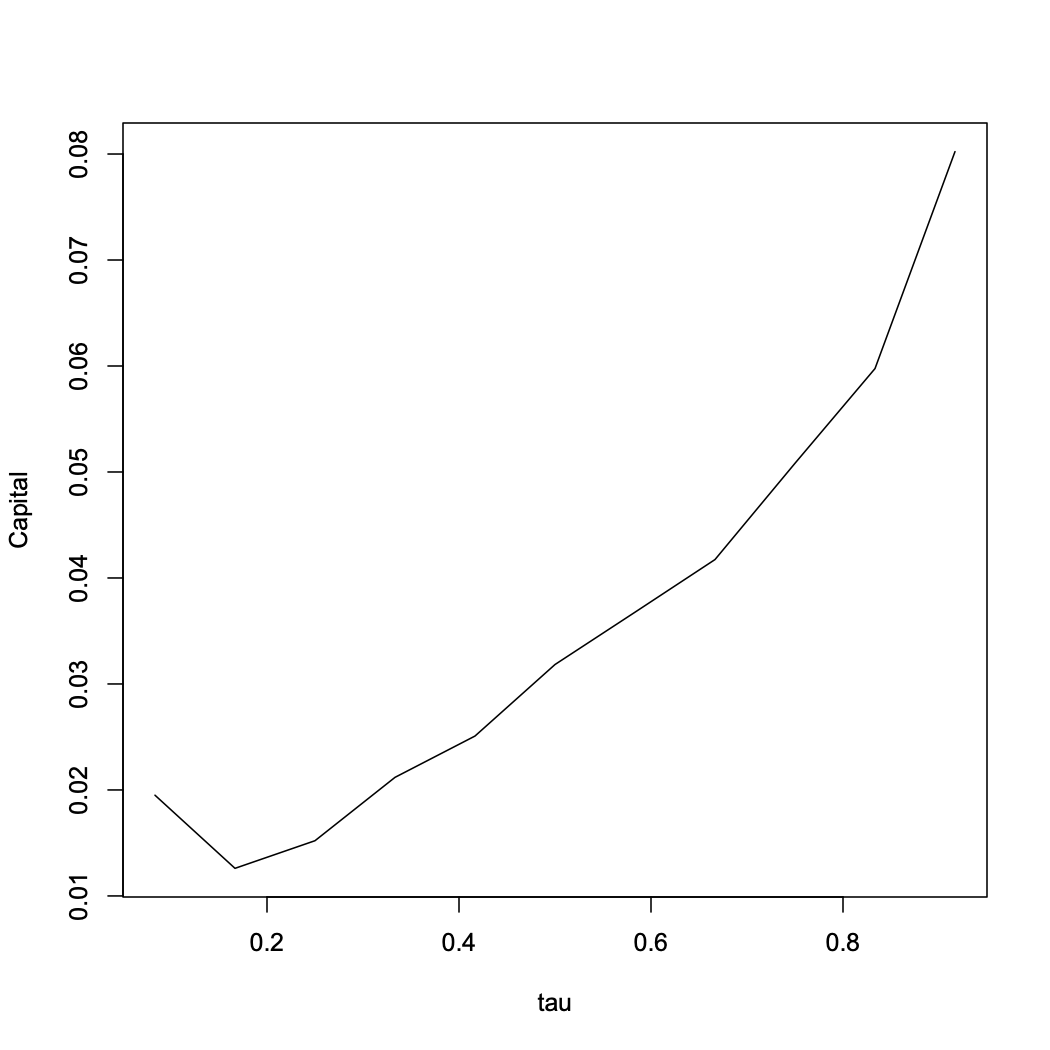
\includegraphics[width=7cm, height=7cm]{/Users/justindoty/Documents/Research/Dissertation/Nonlinear_Production_Function_QR/Code/Empirical/US/capital.png}
\end{figure}
\end{frame}

%------------------------------------------------------------------------------------
\begin{frame}
\frametitle{Preliminary Results: Labor Elasticity}
\begin{figure}[ht]
\centering
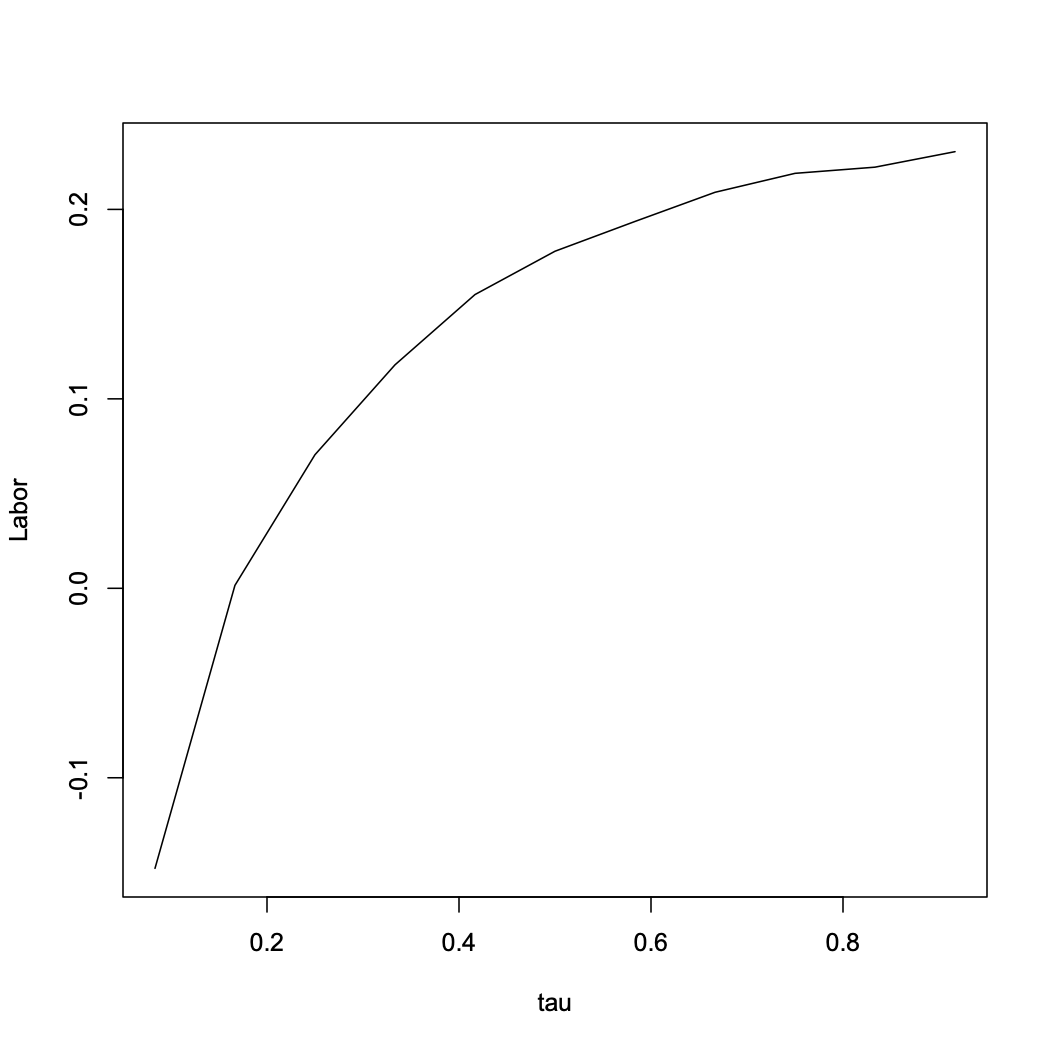
\includegraphics[width=7cm, height=7cm]{/Users/justindoty/Documents/Research/Dissertation/Nonlinear_Production_Function_QR/Code/Empirical/US/labor.png}
\end{figure}
\end{frame}

%------------------------------------------------------------------------------------
\begin{frame}
\frametitle{Preliminary Results: Materials Elasticity}
\begin{figure}[ht]
\centering
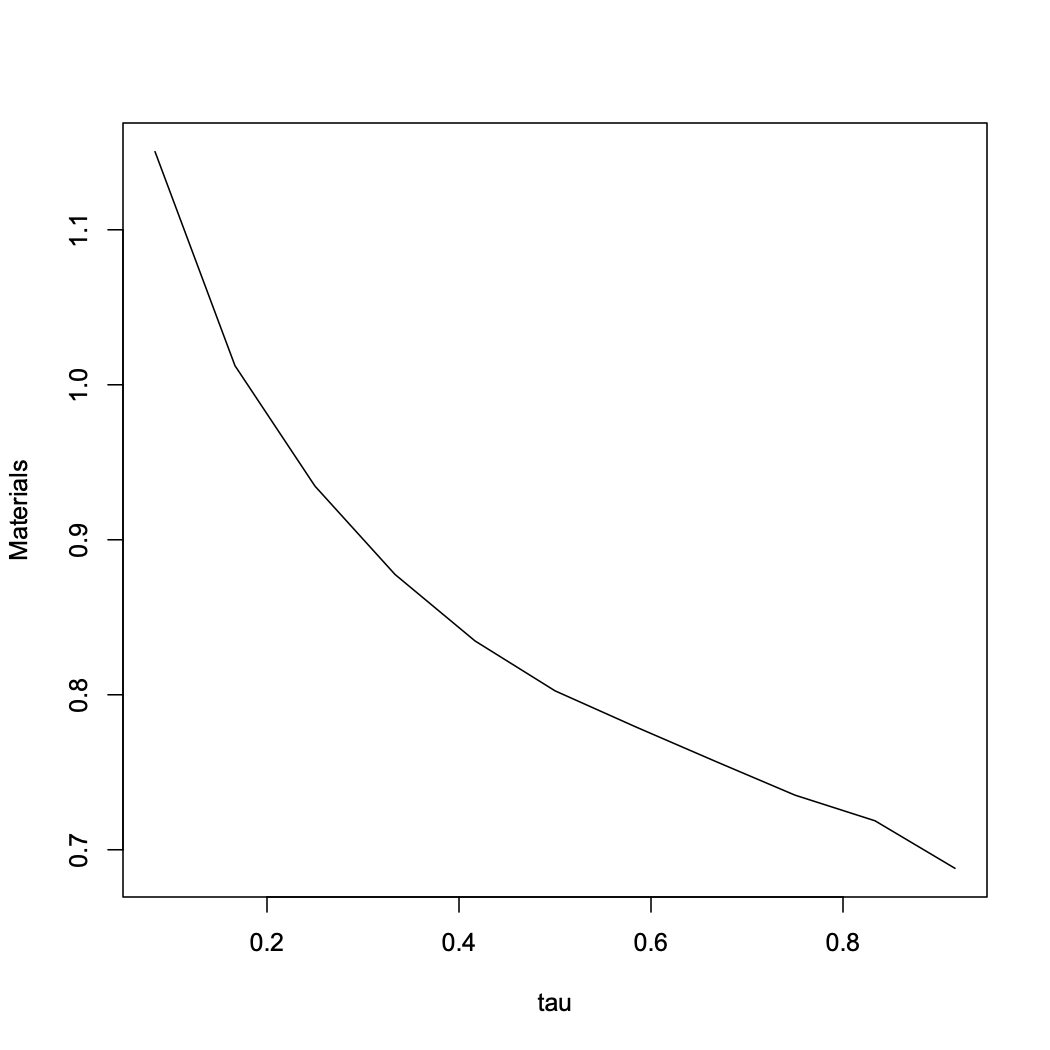
\includegraphics[width=7cm, height=7cm]{/Users/justindoty/Documents/Research/Dissertation/Nonlinear_Production_Function_QR/Code/Empirical/US/materials.png}
\end{figure}
\end{frame}

%------------------------------------------------------------------------------------
\begin{frame}
\frametitle{Preliminary Results: Productivity}
\begin{figure}[ht]
\centering
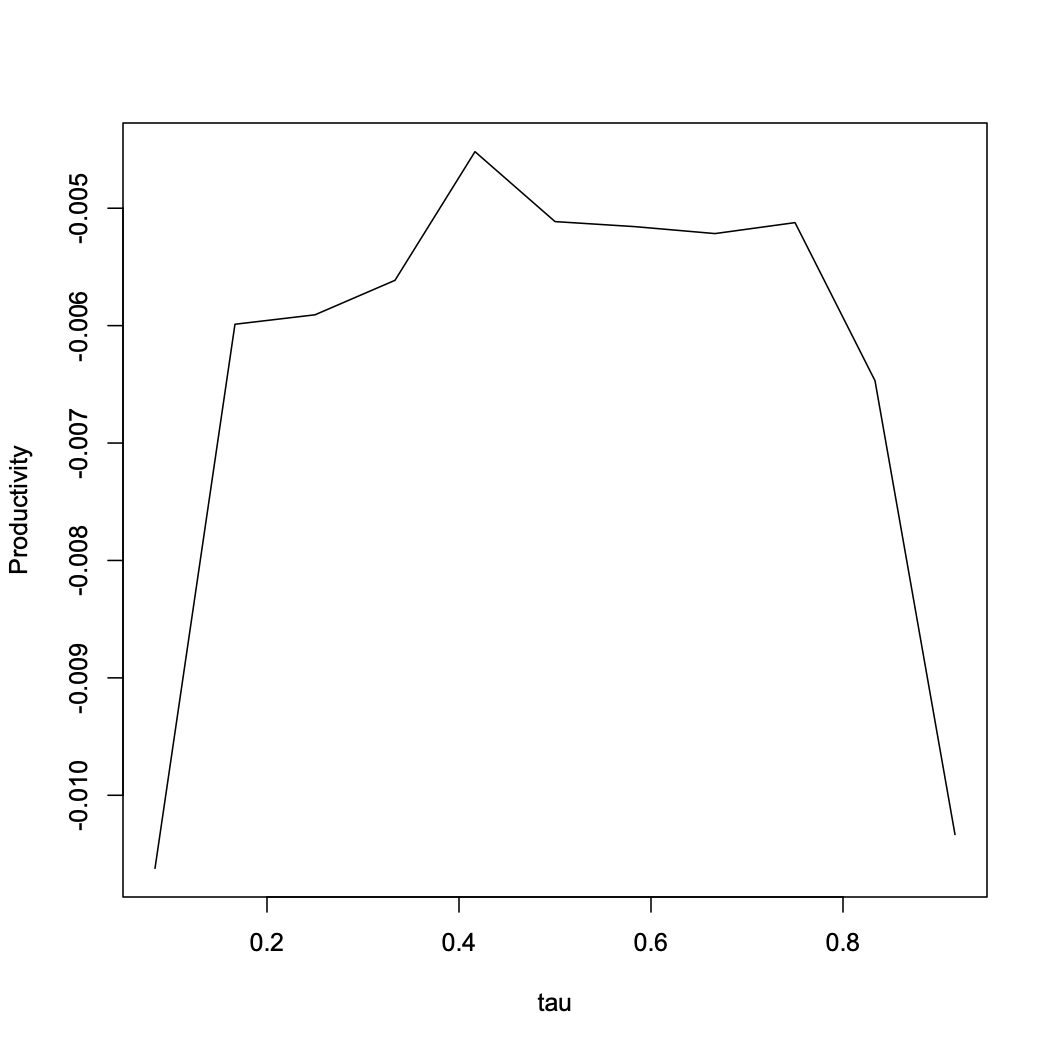
\includegraphics[width=7cm, height=7cm]{/Users/justindoty/Documents/Research/Dissertation/Nonlinear_Production_Function_QR/Code/Empirical/US/productivity.png}
\end{figure}
\end{frame}

%------------------------------------------------------------------------------------
\begin{frame}
\frametitle{Preliminary Results: Average Persistence}
\begin{figure}[ht]
\centering
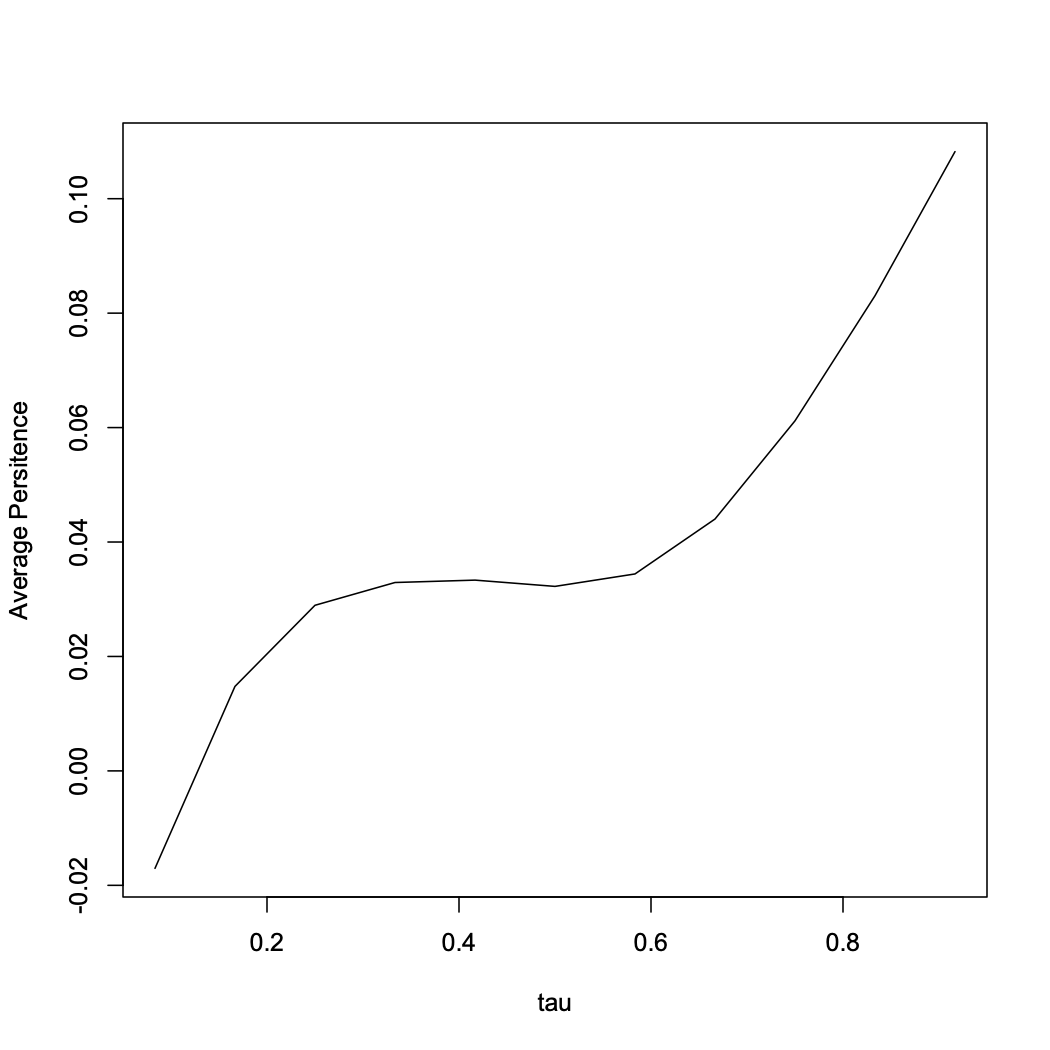
\includegraphics[width=7cm, height=7cm]{/Users/justindoty/Documents/Research/Dissertation/Nonlinear_Production_Function_QR/Code/Empirical/US/pers.png}
\end{figure}
\end{frame}

%------------------------------------------------------------------------------------
\begin{frame}
\frametitle{Preliminary Results: Productivity Distribution}
\begin{figure}[ht]
\centering
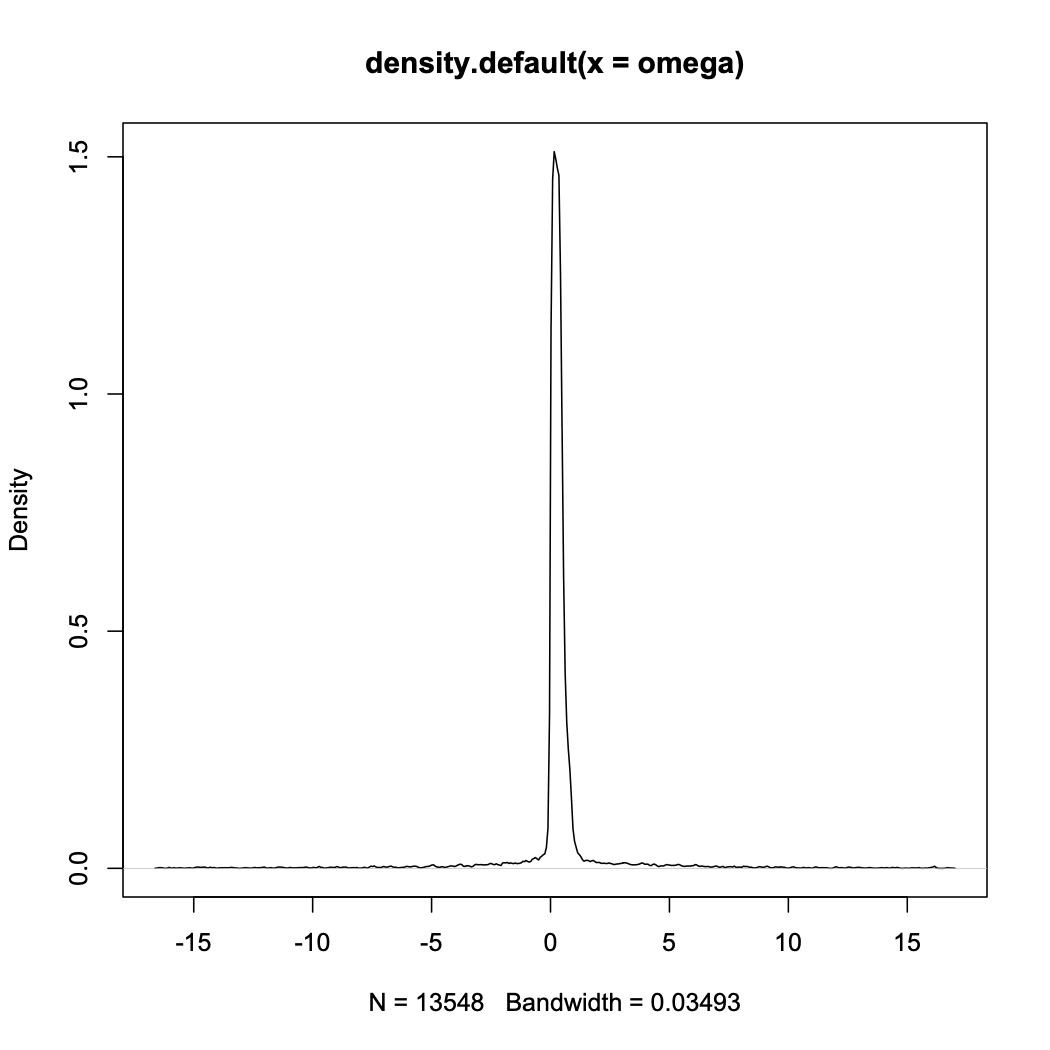
\includegraphics[width=7cm, height=7cm]{/Users/justindoty/Documents/Research/Dissertation/Nonlinear_Production_Function_QR/Code/Empirical/US/dens.png}
\end{figure}
\end{frame}

%------------------------------------------------------------------------------------
\begin{frame}
\frametitle{Addressing a Sample Selection Problem}
\begin{itemize}
	\item Much of the time consumed writing this algorithm was taking into consideration unbalanced panel data
	\item Both \cite{Arellano2016} and \cite{Arellano2017} use balanced panel data in their empirical applications
	\item \cite{Olley1996} address anomalies in production function coefficients estimated from balanced panels. 
	\item They find that going from the balanced sample to the full sample more than doubles the capital coefficient and decreases the labor coefficient by about 20 percent
	\item Productivity is a major determinant of whether or not a plant exits the industry
	\item If firms exit decisions depend on beliefs of future productivity which are partially determined by current productivity then a balanced panel will be selected on the basis of the unobserved productivity realizations
\end{itemize}
\end{frame}


%------------------------------------------------------------------------------------
\begin{frame}
\frametitle{Addressing a Sample Selection Problem}
\begin{itemize}
	\item The exit rule decision is given by
	\begin{equation}
		\chi_{t}=
		\begin{cases}
		1 \quad \text{if}\, \omega_{t}\geq\bar{\omega}_{t}(a_{t}, k_{t})\\
		0 \quad \text{otherwise}
		\end{cases}
	\end{equation}
	where $a_{t}$ denotes another state variable of the firm (age)
	\item Then the second stage of OP
	\begin{equation}
	\begin{split}
	\mathbbm{E}&[y_{it}-\hat{\beta}_{l}l_{it}|\chi_{t}=1, \mathcal{I}_{it}]\\
	&=\beta_{0}+\beta_{k}k_{it}+\beta_{a}a_{it}+\mathbbm{E}[\omega_{it}|\chi_{t}=1, \mathcal{I}_{it}]
	\end{split}
	\end{equation}
	where
	\begin{equation}
	\begin{split}
	\mathbbm{E}[\omega_{it}|\chi_{t}=1, \mathcal{I}_{it}]&=\mathbbm{E}[\omega_{it}|\omega_{t}\geq\bar{\omega}_{t}(a_{t}, k_{t}), \mathcal{I}_{it}]\\
	&\int_{\bar{\omega}_{t}(a_{t}, k_{t})}^{\infty}\omega_{it}\frac{p(\omega_{it}|\omega_{it-1})}{\int_{\bar{\omega}_{t}(a_{t}, k_{t})}^{\infty}p(\omega_{it}|\omega_{it-1})d\omega_{it}}d\omega_{it}\\
	&=g(\omega_{it-1}, \bar{\omega}_{t}(a_{it}, k_{it}))
	\end{split}
	\end{equation}
\end{itemize}
\end{frame}

%------------------------------------------------------------------------------------
\begin{frame}
\frametitle{Addressing a Sample Selection Problem}
\begin{itemize}
	\item In OP, the first stage results conditional on parameters can be used as a proxy for $\omega_{it-1}$
	\item $\bar{\omega}_{t}(a_{it}, k_{it})$ can be controlled using observed data on entry and exit
	\begin{equation}
	\begin{split}
	P(\chi_{t}=1|\mathcal{I}_{it-1})&=P(\omega_{it}\geq\bar{\omega}_{t}(a_{it}, k_{it})|\mathcal{I}_{it-1})\\
	&=\varphi(\omega_{it-1}, \bar{\omega}_{t}(a_{it}, k_{it}))\\
	&=\varphi(\omega_{it-1}, a_{it}, k_{it})\\
	&=\varphi(i_{it-1}, k_{it-1}, a_{it-1})=P_{t}
	\end{split}
	\end{equation}
	which can be nonparametrically estimated using probit with a flexible polynomial of $(i_{it-1}, k_{it-1}, a_{it-1})$ or by using kernel methods
	\item Lastly, we can invert the last line of the above equation to express $\bar{\omega}_{t}(a_{it}, k_{it})$ as a function of $\omega_{it-1}$ and $P_{t}$ so that
	\begin{equation}
	g(\omega_{it-1}, \bar{\omega}_{t}(a_{it}, k_{it}))=\tilde{g}(\omega_{it-1}, P_{t})
	\end{equation}
\end{itemize}
\end{frame}

%------------------------------------------------------------------------------------
\begin{frame}
\frametitle{Addressing a Sample Selection Problem}
\begin{itemize}
	\item Can we apply a similar correction using \cite{Arellano2017a} for quantile models?
	\begin{equation}
	P(\omega_{it}\leq g(\omega_{it-1}, \xi_{it})|\chi_{t}=1, \mathcal{I}_{it-1})=P(\xi_{it}\leq \tau|\bar{\omega}_{t}(a_{it}, k_{it})\leq \omega_{it}, \mathcal{I}_{it-1})
	\end{equation}
	\item They use a copula based method to estimate the dependence between the error in the selection equation and the error in the output equation
	\item Not sure if that method can be applied here or if I should try to see if the OP selection correction can be applied here
	\item This is something to consider in the far future
\end{itemize}
\end{frame}

%------------------------------------------------------------------------------------

\begin{frame}
\frametitle{Conclusion}
\begin{itemize}
	\item Identification strategy is not new, most economists have avoided it due to injectivity assumptions and panel time length requirements
	\item These data requirements become even more stringent if other unobservables (firm fixed effects) are added
	\item Implementation in progress
	\item The estimation procedure is novel and allows us to document a variety of heterogeneous quantile marginal effects, for example, the average quantile marginal effect of labor would be
	\begin{equation}
	\phi_{t}(k_{t}, l_{t}, m_{t}, \tau)=\mathbbm{E}\Bigg[\frac{\partial Q(y_{t}|k_{t}, l_{t}, m_{t}, \omega_{t}, \tau)}{\partial l_{t}}\Bigg]
	\end{equation}
	\item Distributional effects of productivity
	\begin{equation}
	\phi_{t}(k_{t}, l_{t}, m_{t}, \omega_{t}, \tau)=\frac{\partial Q(y_{t}|k_{t}, l_{t}, m_{t}, \omega_{t}, \tau)}{\partial \omega_{t}}
	\end{equation}
\end{itemize}
\end{frame}

%------------------------------------------------------------------------------------

\begin{frame}
\frametitle{Conclusion}
\begin{itemize}
	\item Dynamic effects of innovation shocks on production
	\begin{equation}
	\begin{split}
	\frac{\partial}{\partial \xi_{it}}&\Bigg[\frac{\partial Q(y_{t}|k_{t}, l_{t}, m_{t}, Q_{t}(\omega_{t-1}, \xi_{t}), \tau)}{\partial \omega_{t}}\Bigg]\Bigg|_{\xi=\tau_{\xi}}\\
	&=\phi_{t}(k_{t}, l_{t}, m_{t}, Q_{t}(\omega_{t-1}, \tau_{\xi}), \tau)\frac{\partial Q_{t}(\omega_{t-1}, \tau_{\xi})}{\partial \xi}
	\end{split}
	\end{equation}
	\item ``Impulse response'' functions can be written as
	\begin{equation}
	\frac{\partial}{\partial \omega_{t-1}}\Bigg[\frac{\partial Q_{t}(\omega_{t-1}, \tau_{\xi})}{\partial \xi}\Bigg]
	\end{equation}
	and can be approximated by finite differences across $\tau_{\xi}$ to study the asymmetric impacts of innovation shocks at different points on the output distribution over firm age
	\item Many more interesting effects can be formalized and calculated
\end{itemize}

\end{frame}














\end{document}

